\section{Architettura di sistema}
\subsection{\textit{Data processing architectures}}
Le architetture di tipo \textit{data processing} sono progettate per gestire l'\textit{ingestion}, \textit{processing} e memorizzazione di grandi quantità di dati.
Esse permettono di analizzare e ottenere informazioni utili (\textit{insight}) da questi dati, consentendo di ottimizzare i processi decisionali e migliorare le prestazioni aziendali.
Esistono diverse architettura, ciascuna con le proprie caratteristiche e vantaggi. Tra le più comuni troviamo l'architettura \textit{lambda} e l'architettura \textit{kappa}.

\subsubsection{Architettura \textit{lambda}}
L'architettura \textit{lambda} è costituita dalle seguenti quattro componenti:
\begin{itemize}
	\item \textbf{sorgente di dati}: responsabile dell'acquisizione dei dati grezzi da diverse sorgenti;
	\item \textbf{\textit{batch layer}}: responsabile dell'elaborazione e persistenza di dati storici in \textit{batch} di grandi dimensioni; il suo scopo è fornire risposte complete e accurate, anche se con una latenza più elevata rispetto allo \textit{speed layer}. Tale componente è tipicamente rappresentata da \textit{framework} come Apache Hadoop o Apache Spark;
	\item \textbf{\textit{speed (real-time) layer}}: responsabile dell'elaborazione e persistenza di dati in tempo reale. I dati vengono elaborati in modo rapido e con una latenza molto bassa, fornendo tuttavia risposte elaborate rispetto al \textit{batch layer}. Questa componente è tipicamente rappresentata da \textit{framework} come Apache Storm o Apache Flink;
	\item \textbf{\textit{serving layer}}: responsabile della fornitura dei dati elaborati in modo veloce ed affidabile, indipendentemente dal \textit{layer} di elaborazione utilizzato.
\end{itemize}

\begin{center}
	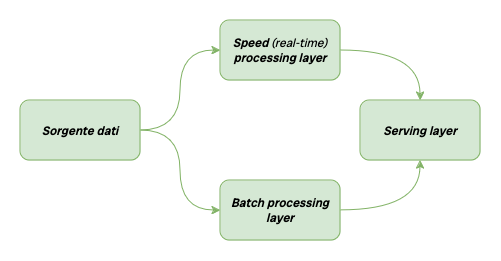
\includegraphics[width=0.6\textwidth]{./specifica_tecnica/architettura_lambda.png}
	\captionof{figure}{Architettura \textit{lambda}}
\end{center}

\subsubsubsection{Vantaggi e svantaggi}
L'architettura \textit{lambda} offre diversi vantaggi, tra cui la \textbf{scalabilità orizzontale}, la \textbf{tolleranza ai guasti} e la \textbf{flessibilità}. Tuttavia, la presenza
di due \textit{layer} di elaborazione separati può portare a problemi di coerenza dei dati, duplicazione della logica di aggregazione e complessità aggiuntiva nella gestione del sistema.
Inoltre, rispetto all'architettura \textit{kappa}, l'architettura \textit{lambda} può avere una latenza più elevata.

\subsubsubsection{Casi d'uso}
L'architettura \textit{lambda} è particolarmente adatta per applicazioni che richiedono sia un'analisi sui dati in tempo reale che un'analisi storica.

\subsubsection{Architettura \textit{kappa}}
L'architettura \textit{kappa} è stata introdotta per semplificare l'architettura \textit{lambda}, eliminando la necessità di gestire due \textit{layer} di elaborazione separati per il \textit{batch processing} e il \textit{real-time processing}.
Essa si divide in tre componenti principali:
\begin{itemize}
	\item \textbf{sorgente di dati}: responsabile dell'acquisizione dei dati grezzi da diverse sorgenti;
	\item \textbf{\textit{processing layer}}: responsabile dell'elaborazione dei dati in tempo reale, senza la necessità di separare i dati in \textit{batch} e \textit{real-time};
	\item \textbf{\textit{serving layer}}: responsabile della fornitura dei dati elaborati in modo veloce ed affidabile.
\end{itemize}

\begin{center}
	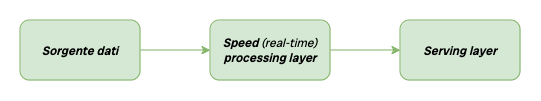
\includegraphics[width=0.6\textwidth]{./specifica_tecnica/architettura_kappa.png}
	\captionof{figure}{Architettura \textit{kappa}}
\end{center}

\subsubsubsection{Vantaggi e svantaggi}
L'architettura \textit{kappa} offre diversi vantaggi, tra cui la \textbf{semplicità}, la \textbf{riduzione dei costi} e la \textbf{bassa latenza}.
Tuttavia, può non essere adatta per applicazioni che richiedono un'analisi storica dei dati.

\subsubsubsection{Casi d'uso}
L'architettura \textit{kappa} è particolarmente adatta per gli scenari in cui sono critici i dati in tempo reale e l'analisi dei dati storici è meno importante. Inoltre, semplifica notevolmente il processo di sviluppo e manutenzione dei sistemi di elaborazione dei dati.

\subsection{Architettura scelta}
Nello scenario del capitolato proposto da \textit{SyncLab S.r.L.}, è importante l'analisi in tempo reale, in quanto i dati provenienti dai sensori IoT devono fornire informazioni sempre aggiornate ed eventualmente
sollevare allarmi in caso di situazioni critiche. Inoltre, non è richiesta l'aggregazione storica di dati, dunque i vantaggi dell'architettura \textit{lambda} non risultano utili per i nostri fini.
Per soddisfare tali requisiti, è stata dunque scelta l'architettura \textit{kappa}.

\subsubsection{Componenti di sistema}
All'interno del sistema progettato sono dunque presenti le seguenti componenti:
\begin{itemize}
	\item \textbf{sorgenti di dati}: costituite dal simulatore di sensori, il quale genera i dati grezzi che in un contesto reale sarebbero provenienti dai sensori IoT;
	\item \textbf{\textit{streaming layer}}: gestisce il flusso di dati in tempo reale provenienti dai sensori. È composto da \textit{Redpanda} e lo \textit{Schema Registry};
	\item \textbf{\textit{processing layer}}: elabora i dati in tempo reale per calcolare metriche e indici. È composto da \textit{Apache Flink};
	\item \textbf{\textit{storage layer}}: memorizza i dati elaborati per l'analisi e la visualizzazione. È composto da \textit{ClickHouse};
	\item \textbf{\textit{data visualization layer}}: fornisce un'interfaccia utente per visualizzare i dati elaborati. È composto da \textit{Grafana}.
\end{itemize}

\begin{center}
	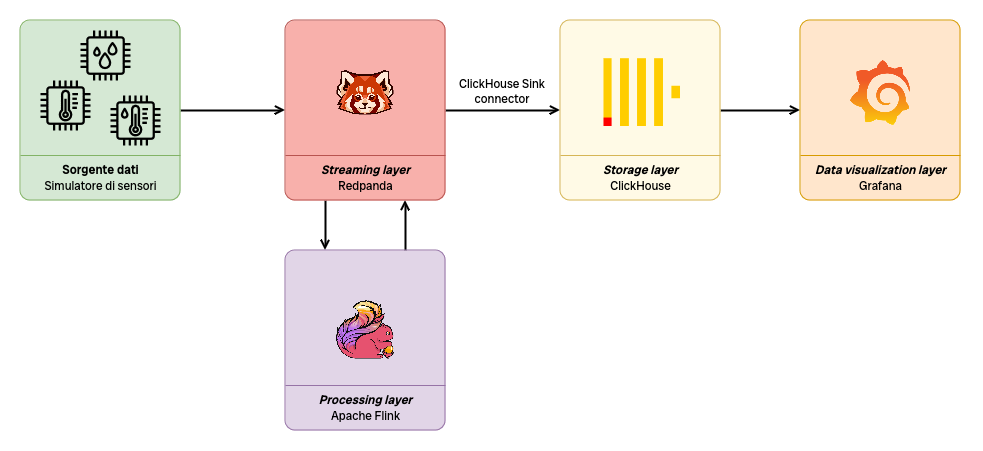
\includegraphics[width=0.7\textwidth]{./specifica_tecnica/architettura_sistema.png}
	\captionof{figure}{Componenti di sistema ad alto livello}
\end{center}

\subsubsection{Flusso di dati}
Per illustrare il flusso di dati all'interno del sistema, è stato realizzato il seguente diagramma, il quale mostra il percorso che i dati grezzi seguono dal simulatore fino alla visualizzazione tramite Grafana.
\begin{center}
	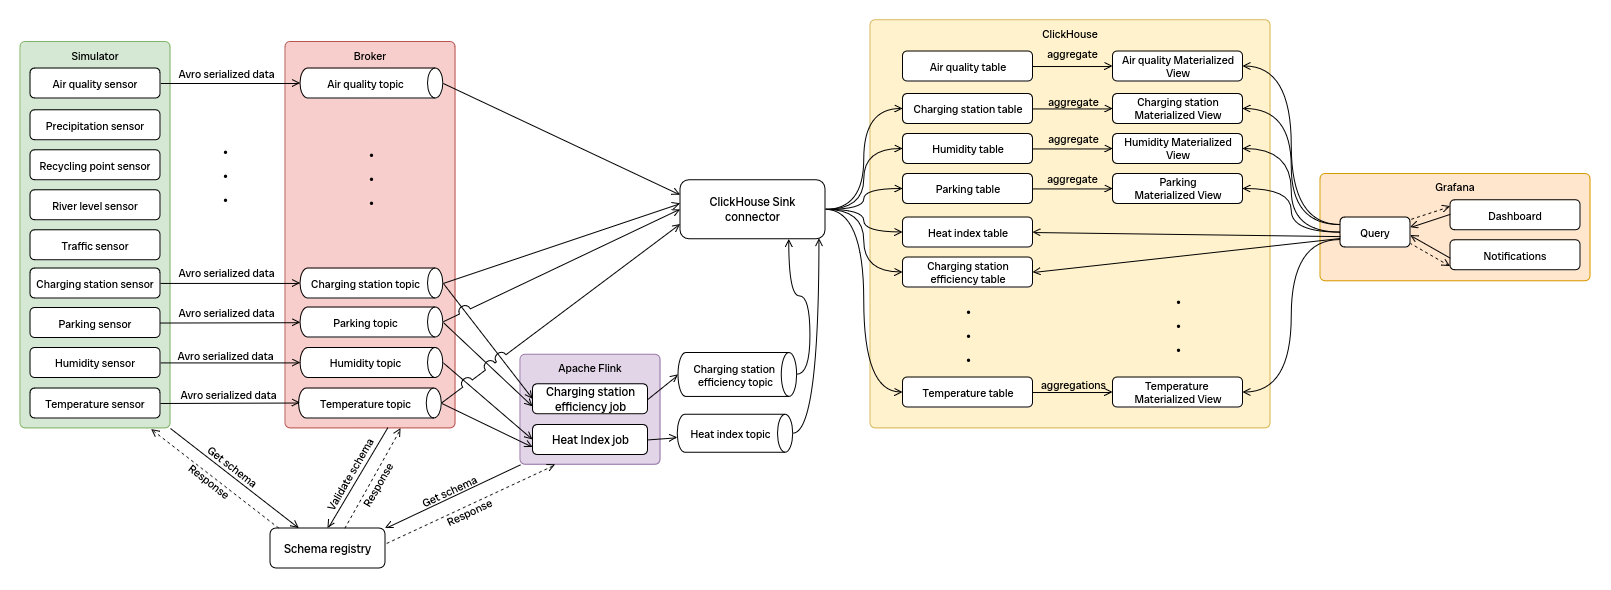
\includegraphics[width=1\textwidth]{./specifica_tecnica/data_flow.png}
	\captionof{figure}{Flusso di dati all'interno del sistema. I sensori di precipitazioni, isole ecologiche, livello dei fiumi e traffico sono stati omessi per chiarezza, ma il percorso di tali dati è analogo a quello dei sensori di qualità dell'aria.}
\end{center}

Il flusso seguito dai dati si può riassumere nei seguenti passaggi:
\begin{enumerate}
	\item \textbf{generazione dei dati}: ciascun simulatore emula il comportamento di un singolo sensore IoT, generando ad intervalli periodici o ad eventi (\textit{event-driven}) i dati grezzi relativi alla propria tipologia di dato.
	\item \textbf{serializzazione e produzione dei dati}: i dati grezzi generati nel punto precedente vengono serializzati utilizzando il formato Confluent Avro e inviati nel \textit{topic} corrispondente al tipo di dato generato;
	\item \textbf{elaborazione dei dati}: i \textit{topic} contenenti i dati grezzi di temperatura, umidità, occupazione dei parcheggi e colonnine di ricarica vengono consumati da Apache Flink.
	      Due \textit{job} distinti si occupano di calcolare la temperatura percepita e il grado di efficienza delle colonnine di ricarica. Una volta elaborati, i dati vengono inviati rispettivamente
	      nei \textit{topic} \texttt{heat\_index} e \texttt{charging\_station\_efficiency};
	\item \textbf{memorizzazione dei dati}: attraverso il connettore \textit{sink} per ClickHouse, i dati pubblicati in tutti i \textit{topic} vengono memorizzati nel database;
	\item \textbf{aggregazioni con \textit{materialized view}}: attraverso l'utilizzo di \textit{materialized view} in ClickHouse, vengono calcolate le statistiche relative ai dati memorizzati, come ad esempio la media oraria o giornaliera.
	      Tali aggregazioni sono più semplici rispetto a quelle effettuate da Flink, in quanto non richiedono elaborazioni complesse sui dati;
	\item \textbf{visualizzazione dei dati}: i dati memorizzati in ClickHouse vengono visualizzati tramite Grafana, che permette di creare \textit{dashboard} personalizzate per monitorare i dati in tempo reale;
	\item \textbf{notifiche}: Grafana esegue periodicamente delle \textit{query} per verificare se sono state superate delle soglie predeterminate. In caso affermativo, vengono inviate notifiche tramite il canale Discord dedicato, in modo tale da poter avvisare l'autorità locale.
\end{enumerate}

\subsection{Architettura dei simulatori}
I simulatori vengono utilizzati per produrre dati grezzi che sostituiscono le rilevazioni effettuate dai sensori IoT in un contesto reale.
Per tale motivo, questa parte del sistema non è ufficialmente parte del prodotto finale, ma è stata sviluppata per scopi di \textit{test}
e dimostrativi nell'ambito del progetto didattico; ai fini di quest'ultimo, il gruppo ha deciso di dedicare alcune risorse per la progettazione.\\
Nei paragrafi successivi verranno descritti i moduli che compongono i simulatori, le classi e metodi principali e i \textit{design pattern} utilizzati.\\
Sono stati implementati simulatori per i seguenti tipi dato:
\begin{itemize}
	\item qualità dell'aria;
	\item precipitazioni;
	\item isole ecologiche;
	\item livello dei fiumi;
	\item traffico;
	\item colonnine di ricarica;
	\item parcheggi;
	\item temperatura;
	\item umidità.
\end{itemize}

\subsubsection{Modulo \texttt{models}}
Questo modulo contiene le classi che rappresentano i dati grezzi generati dai sensori (sottomodulo \texttt{raw\_data}) e la configurazione dei sensori stessi (sottomodulo \texttt{config}) letta
dal file di configurazione \texttt{sensors.toml} e dalle variabili d'ambiente.\\
Ciascun tipo di dato grezzo è rappresentato da una classe che estende \texttt{RawData} (astratta).\\
La classe \texttt{SensorConfig} riceve nel costruttore la configurazione sotto forma di dizionario, effettua \textit{parsing}, validazione,
popola con valori di \textit{default} i campi mancanti (nel caso lo prevedano) ed inizializza i propri attributi, corrispondenti ai campi del file di configurazione.\\
Allo stesso modo, \texttt{EnvConfig} legge le variabili d'ambiente ed espone il metodo \texttt{bootstrap\_server()} che combina \textit{host} e \textit{port} per formare l'indirizzo del \textit{broker} Kafka.\\
\begin{center}
	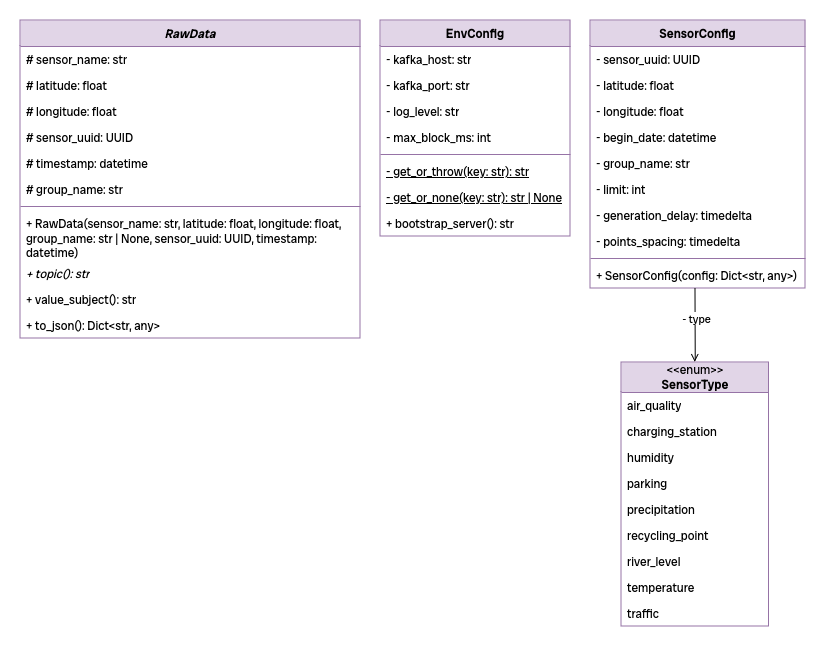
\includegraphics[width=0.87\textwidth]{./specifica_tecnica/models.png}
	\captionof{figure}{Diagramma delle classi del modulo \texttt{models}. Per ragioni di spazio, le implementazioni di \texttt{RawData} sono illustrate nel diagramma successivo}
\end{center}

\subsubsubsection{Classi, interfacce metodi e attributi}
\begin{itemize}
	\item \textbf{Classe astratta \texttt{RawData}}:
	      \begin{itemize}
		      \item \textbf{Attributi}
		            \begin{itemize}
			            \item \texttt{sensor\_uuid} string [protected]: identificativo univoco del sensore;
			            \item \texttt{latitude} float [protected]: latitudine del sensore;
			            \item \texttt{longitude} float [protected]: longitudine del sensore;
			            \item \texttt{sensor\_name} string [protected]: nome del sensore;
			            \item \texttt{group\_name} string [protected]: nome del gruppo di sensori a cui appartiene.
		            \end{itemize}
		      \item \textbf{Metodi}
		            \begin{itemize}
			            \item \texttt{topic()} string [public,abstract]: restituisce il nome del \textit{topic} in cui i dati grezzi vanno pubblicati;
			            \item \texttt{value\_subject()} string [public]: restituisce il nome del campo value del record.
		            \end{itemize}
	      \end{itemize}
	\item \textbf{Classe EnvConfig}:
	      \begin{itemize}
		      \item \textbf{Attributi}
		            \begin{itemize}
			            \item \texttt{kafka\_host} string [private]: \textit{host} del \textit{broker} Kafka;
			            \item \texttt{kafka\_port} string [private]: porta del \textit{broker} Kafka;
			            \item \texttt{log\_level} string [private]: livello di \textit{logging} da utilizzare;
			            \item \texttt{max\_block\_ms} int [private]: tempo massimo di blocco per la produzione di messaggi.
		            \end{itemize}
		      \item \textbf{Metodi}
		            \begin{itemize}
			            \item \texttt{get\_or\_throw(key: string)} string [private,static]: restituisce il valore della variable d'ambiente associato alla chiave \texttt{key} se presente, altrimenti lancia un'eccezione;
			            \item \texttt{get\_or\_none(key: string)} string [private,static]: restituisce il valore della variable d'ambiente associato alla chiave \texttt{key} se presente, altrimenti \texttt{None};
			            \item \texttt{bootstrap\_server()} string [public]: restituisce l'indirizzo del \textit{broker} Kafka.
		            \end{itemize}
	      \end{itemize}
	\item \textbf{Classe SensorConfig}:
	      \begin{itemize}
		      \item \textbf{Attributi}
		            \begin{itemize}
			            \item \texttt{sensor\_uuid} string [private]: identificativo univoco del sensore;
			            \item \texttt{limit} int [private]: limite massimo di misurazioni da effettuare;
			            \item \texttt{begin\_date} datetime [private]: data e ora di inizio delle misurazioni;
			            \item \texttt{latitude} float [private]: latitudine del sensore;
			            \item \texttt{longitude} float [private]: longitudine del sensore;
			            \item \texttt{group\_name} string [private]: nome del gruppo di sensori a cui appartiene;
			            \item \texttt{type} SensorType [private]: tipo di sensore;
			            \item \texttt{points\_spacing} timedelta [private]: intervallo temporale tra due misurazioni;
			            \item \texttt{generation\_delay} timedelta [private]: ritardo tra la generazione di due misurazioni adiacenti.
		            \end{itemize}
	      \end{itemize}
	\item \textbf{Enum SensorType}:
	      \begin{itemize}
		      \item \textbf{Valori}
		            \begin{itemize}
			            \item \texttt{AIR\_QUALITY}
			            \item \texttt{PARKING}
			            \item \texttt{RECYCLING\_POINT}
			            \item \texttt{TEMPERATURE}
			            \item \texttt{TRAFFIC}
			            \item \texttt{CHARGING\_STATION}
			            \item \texttt{PRECIPITATION}
			            \item \texttt{RIVER\_LEVEL}
			            \item \texttt{HUMIDITY}
		            \end{itemize}
		      \item \textbf{Metodi}
		            \begin{itemize}
			            \item \texttt{from\_str(value: string)} SensorType [public,static]: restituisce il valore dell'enum corrispondente alla stringa \texttt{value}.
		            \end{itemize}
	      \end{itemize}
	\item \textbf{Classe AirQualityRawData}
	      \begin{itemize}
		      \item \textbf{Metodi}:
		            \begin{itemize}
			            \item \texttt{topic()} str [public]: restituisce il nome del \textit{topic} in cui i dati grezzi vanno pubblicati.
		            \end{itemize}
	      \end{itemize}
	\item \textbf{Classe ChargingStationRawData}
	      \begin{itemize}
		      \item \textbf{Metodi}:
		            \begin{itemize}
			            \item \texttt{topic()} str [public]: restituisce il nome del \textit{topic} in cui i dati grezzi vanno pubblicati.
		            \end{itemize}
	      \end{itemize}
	\item \textbf{Classe HumidityRawData}
	      \begin{itemize}
		      \item \textbf{Metodi}:
		            \begin{itemize}
			            \item \texttt{topic()} str [public]: restituisce il nome del \textit{topic} in cui i dati grezzi vanno pubblicati.
		            \end{itemize}
	      \end{itemize}
	\item \textbf{Classe ParkingRawData}
	      \begin{itemize}
		      \item \textbf{Metodi}:
		            \begin{itemize}
			            \item \texttt{topic()} str [public]: restituisce il nome del \textit{topic} in cui i dati grezzi vanno pubblicati.
		            \end{itemize}
	      \end{itemize}
	\item \textbf{Classe PrecipitationRawData}
	      \begin{itemize}
		      \item \textbf{Metodi}:
		            \begin{itemize}
			            \item \texttt{topic()} str [public]: restituisce il nome del \textit{topic} in cui i dati grezzi vanno pubblicati.
		            \end{itemize}
	      \end{itemize}
	\item \textbf{Classe RecyclingPointRawData}
	      \begin{itemize}
		      \item \textbf{Metodi}:
		            \begin{itemize}
			            \item \texttt{topic()} str [public]: restituisce il nome del \textit{topic} in cui i dati grezzi vanno pubblicati.
		            \end{itemize}
	      \end{itemize}
	\item \textbf{Classe RiverLevelRawData}
	      \begin{itemize}
		      \item \textbf{Metodi}:
		            \begin{itemize}
			            \item \texttt{topic()} str [public]: restituisce il nome del \textit{topic} in cui i dati grezzi vanno pubblicati.
		            \end{itemize}
	      \end{itemize}
	\item \textbf{Classe TemperatureRawData}
	      \begin{itemize}
		      \item \textbf{Metodi}:
		            \begin{itemize}
			            \item \texttt{topic()} str [public]: restituisce il nome del \textit{topic} in cui i dati grezzi vanno pubblicati.
		            \end{itemize}
	      \end{itemize}
	\item \textbf{Classe TrafficRawData}
	      \begin{itemize}
		      \item \textbf{Metodi}:
		            \begin{itemize}
			            \item \texttt{topic()} str [public]: restituisce il nome del \textit{topic} in cui i dati grezzi vanno pubblicati.
		            \end{itemize}
	      \end{itemize}
\end{itemize}

\subsubsection{Modulo \texttt{simulators}}
Il modulo \texttt{simulators} contiene la logica per la generazione dei dati grezzi e l'orchestrazione dei simulatori.\\
L'\textit{entrypoint} di tutto il sistema è la classe \texttt{SimulatorExecutor}, che riceve la configurazione dei sensori
ed utilizzando il \texttt{SimulatorFactory} crea un \texttt{SimulatorThread} per ogni sensore.
Quest'ultimo, a partire da una \texttt{SimulatorStrategy} ed una \texttt{ProducerStrategy}, genera i dati grezzi e li invia al \texttt{Producer}.\\
La classe \texttt{SimulatorThread} utilizza un \texttt{threading.Event}, che contiene un \textit{flag} booleano.
Quest'ultimo può essere impostato a \texttt{True} per far partire il \textit{thread}; il metodo \texttt{wait()} permette di mettere in attesa il \textit{thread} fino a quando il \textit{flag} è
impostato a \texttt{True}, per un periodo di tempo massimo espresso dal parametro \texttt{timeout}.\\ Tale metodo è utilizzato per attendere un determinato periodo di tempo tra la generazione di due misurazioni.\\

\begin{center}
	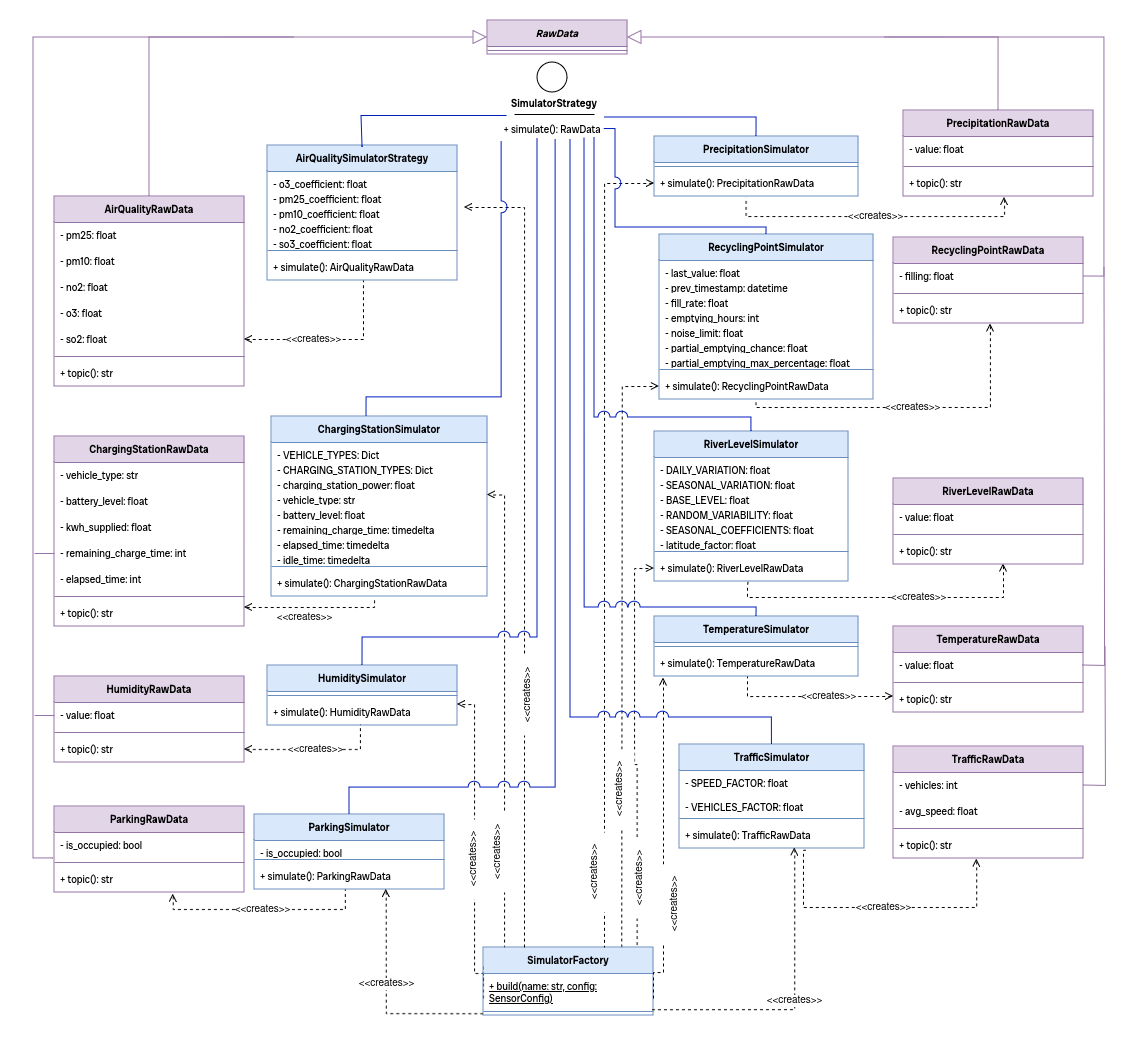
\includegraphics[width=1\textwidth]{./specifica_tecnica/simulators.png}
	\captionof{figure}{Diagramma delle classi modulo \texttt{simulators} e \texttt{models}. Per semplicità e chiarezza, la classe \texttt{SimulatorFactory} è stata rappresentata senza campi e metodi, presenti nel diagramma successivo.}
\end{center}

\subsubsubsection{\textit{Design Pattern}}
\subsubsubsubsection{\textit{Strategy}}
All'interno del modulo \texttt{simulators} è stato utilizzato il \textit{design pattern} \textit{Strategy} per permettere la generazione di dati grezzi di diversi tipi.
Ciascuna tipologia simulatore implementa l'interfaccia \texttt{SimulatorStrategy} che definisce il metodo \texttt{simulate()}. In questo modo, la classe \texttt{SimulatorThread}
può eseguire il simulatore senza conoscere il tipo di dato generato, rendendo inoltre semplice l'aggiunta di nuovi tipi di dati grezzi senza dover modificare il codice esistente.

\subsubsubsubsection{\textit{Factory}}
La classe \texttt{SimulatorFactory} implementa il \textit{design pattern} \textit{Factory}, fornendo un metodo che si occupa della creazione dei simulatori
a partire da un valore dell'enum \texttt{SensorType}.


\subsubsubsection{Classi, interfacce metodi e attributi}
\begin{itemize}
	\item \textbf{Classe SimulatorExecutor}
	      \begin{itemize}
		      \item \textbf{Attributi}:
		            \begin{itemize}
			            \item \texttt{simulator\_threads} List[SimulatorThread] [private]: lista dei simulatori da eseguire;
			            \item \texttt{stop\_event}: threading.Event [private]: evento utilizzato per tenere attivo il \textit{thread} principale dopo aver lanciato i \textit{thread} dei simulatori.
		            \end{itemize}
		      \item \textbf{Metodi}:
		            \begin{itemize}
			            \item \texttt{stop\_all()} None [public]:
			            \item \texttt{run()} None [public]:
		            \end{itemize}
	      \end{itemize}
	\item \textbf{Classe SimulatorFactory}
	      \begin{itemize}
		      \item \textbf{Metodi}:
		            \begin{itemize}
			            \item \texttt{build(name: str, config: SensorConfig, producer: ProducerStrategy)} SimulatorStrategy [public, static]: restituisce un'istanza del simulatore \\ corrispondente al nome \texttt{name}.
		            \end{itemize}
	      \end{itemize}
	\item \textbf{Interfaccia SimulatorStrategy}
	      \begin{itemize}
		      \item \textbf{Attributi}:
		            \begin{itemize}
			            \item \texttt{generation\_delay} timedelta [protected]: ritardo tra la generazione di due misurazioni adiacenti.
			            \item \texttt{group\_name} str [protected]: nome del gruppo di sensori a cui appartiene il sensore;
			            \item \texttt{latitude} float [protected]: latitudine del sensore;
			            \item \texttt{limit} int [protected]: limite massimo di misurazioni da produrre;
			            \item \texttt{longitude} float [protected]: longitudine del sensore;
			            \item \texttt{points\_spacing} timedelta [protected]: intervallo temporale tra due misurazioni;
			            \item \texttt{producer} ProducerStrategy [protected]: strategia di produzione dei dati.
			            \item \texttt{sensor\_name} str [protected]: nome del sensore per cui il simulatore genera dati;
			            \item \texttt{sensor\_uuid} str [protected]: identificativo univoco del sensore per cui il simulatore genera dati;
			            \item \texttt{timestamp} datetime [protected]: data e ora dell'ultima misurazione;
		            \end{itemize}
		      \item \textbf{Metodi}:
		            \begin{itemize}
			            \item \texttt{simulate} RawData [public]: metodo che simula la generazione di dati grezzi;
		            \end{itemize}
	      \end{itemize}
	\item \textbf{Classe SimulatorThread}
	      \begin{itemize}
		      \item \textbf{Attributi}:
		            \begin{itemize}
			            \item \texttt{simulator} SimulatorStrategy [private]: simulatore da eseguire;
			            \item \texttt{event} threading.Event [private]: evento utilizzato per fermare, far partire o lasciare in attesa il \textit{thread} del simulatore.
		            \end{itemize}
		      \item \textbf{Metodi}:
		            \begin{itemize}
			            \item \texttt{run()} None [public]: esegue il simulatore;
			            \item \texttt{is\_running()} bool [public]: restituisce \texttt{True} se il \textit{thread} è in esecuzione, \texttt{False} altrimenti;
			            \item \texttt{stop()} None [public]: ferma il \textit{thread} del simulatore.
		            \end{itemize}
	      \end{itemize}
	\item \textbf{Classe AirQualitySimulatorStrategy}
	      \begin{itemize}
		      \item \textbf{Attributi}:
		            \begin{itemize}
			            \item \texttt{o3\_coefficient} float [private]: coefficiente randomico utilizzato per generare il valore di \texttt{o3};
			            \item \texttt{pm25\_coefficient} float [private]: coefficiente randomico utilizzato per generare il valore di \texttt{pm25};
			            \item \texttt{pm10\_coefficient} float [private]: coefficiente randomico utilizzato per generare il valore di \texttt{pm10};
			            \item \texttt{no2\_coefficient} float [private]: coefficiente randomico utilizzato per generare il valore di \texttt{no2};
			            \item \texttt{so2\_coefficient} float [private]: coefficiente randomico utilizzato per generare il valore di \texttt{so2};
		            \end{itemize}
		      \item \textbf{Metodi}:
		            \begin{itemize}
			            \item \texttt{simulate()} AirQualityRawData [public]: genera un dato di tipo AirQualityRawData;
		            \end{itemize}
	      \end{itemize}
	\item \textbf{Classe ChargingStationSimulatorStrategy}
	      \begin{itemize}
	      \end{itemize}
	      \begin{itemize}
		      \item \textbf{Attributi}:
		            \begin{itemize}
			            \item \texttt{VEHICLE\_TYPES}: Dict[str, Dict[str, float]] [private]: dizionario contenente i tipi di veicoli supportati e la capacità minima e massima della batteria;
			            \item \texttt{CHARGING\_STATION\_TYPES} Dict[str, Dict[str, float]] [private]: dizionario contenente i tipi di colonnine di ricarica supportati e la potenza minima e massima;
			            \item \texttt{charging\_station\_power} float [private]: potenza della colonnina di ricarica;
			            \item \texttt{vehicle\_type} str [private]: tipo di veicolo supportato dalla colonnina di ricarica;
			            \item \texttt{battery\_level} float [private]: livello di carica della batteria;
			            \item \texttt{remaining\_charge\_time} timedelta [private]: tempo rimanente per completare la ricarica;
			            \item \texttt{elapsed\_time} timedelta [private]: tempo trascorso dall'inizio della ricarica;
			            \item \texttt{idle\_time} timedelta [private]: tempo in cui la colonnina di ricarica è inattiva;
		            \end{itemize}
		      \item \textbf{Metodi}:
		            \begin{itemize}
			            \item \texttt{simulate()} ChargingStationRawData [public]: genera un dato di
			                  tipo \\ChargingStationRawData;
		            \end{itemize}
	      \end{itemize}
	\item \textbf{Classe HumiditySimulatorStrategy}
	      \begin{itemize}
		      \item \textbf{Metodi}:
		            \begin{itemize}
			            \item \texttt{simulate()} HumidityRawData [public]: genera un dato di tipo HumidityRawData;
		            \end{itemize}
	      \end{itemize}
	\item \textbf{Classe ParkingSimulatorStrategy}
	      \begin{itemize}
		      \item \textbf{Attributi}:
		            \begin{itemize}
			            \item \texttt{is\_occupied} bool [private]: indica se il parcheggio è occupato;
		            \end{itemize}
		      \item \textbf{Metodi}:
		            \begin{itemize}
			            \item \texttt{simulate()} ParkingRawData [public]: genera un dato di tipo ParkingRawData;
		            \end{itemize}
	      \end{itemize}
	\item \textbf{Classe PrecipitationSimulatorStrategy}
	      \begin{itemize}
		      \item \textbf{Metodi}:
		            \begin{itemize}
			            \item \texttt{simulate()} PrecipitationRawData [public]: genera un dato di tipo\\ PrecipitationRawData;
		            \end{itemize}
	      \end{itemize}
	\item \textbf{Classe RecyclingPointSimulatorStrategy}
	      \begin{itemize}
		      \item \textbf{Attributi}:
		            \begin{itemize}
			            \item \texttt{last\_value} float [private]: ultimo valore generato;
			            \item \texttt{prev\_timestamp} datetime [private]: data e ora dell'ultima misurazione;
			            \item \texttt{fill\_rate} float [private]: tasso di riempimento del contenitore;
			            \item \texttt{emptying\_hours} int [private]: ore necessarie per svuotare il contenitore;
			            \item \texttt{noise\_limit} float [private]: quantità massima di rumore da aggiungere al valore generato;
			            \item \texttt{partial\_emptying\_chance} float [private]: probabilità di svuotamento parziale;
			            \item \texttt{partial\_emptying\_max\_percentage} float [private]: percentuale massima di svuotamento parziale;
		            \end{itemize}
		      \item \textbf{Metodi}:
		            \begin{itemize}
			            \item \texttt{simulate()} RecyclingPointRawData [public]: genera un dato di tipo\\ RecyclingPointRawData;
		            \end{itemize}
	      \end{itemize}
	\item \textbf{Classe RiverLevelSimulatorStrategy}
	      \begin{itemize}
	      \end{itemize}
	      \begin{itemize}
		      \item \textbf{Attributi}:
		            \begin{itemize}
			            \item \texttt{DAILY\_VARIATION} float [private]: variazione giornaliera massima del livello del fiume;
			            \item \texttt{SEASONAL\_VARIATION} float [private]: variazione stagionale massima del livello del fiume;
			            \item \texttt{BASE\_LEVEL} float [private]: livello base del fiume;
			            \item \texttt{RANDOM\_VARIABILITY} float [private]: massima variazione casuale del livello del fiume;
			            \item \texttt{SEASONAL\_COEFFICIENTS} Dict[int, float] [private]: coefficienti stagionali per la variazione del livello del fiume;
			            \item \texttt{latitude\_factor} float [private]: fattore moltiplicativo per la latitudine;
		            \end{itemize}
		      \item \textbf{Metodi}:
		            \begin{itemize}
			            \item \texttt{simulate()} RiverLevelRawData [public]: genera un dato di tipo RiverLevelRawData;
		            \end{itemize}
	      \end{itemize}
	\item \textbf{Classe TemperatureSimulatorStrategy}
	      \begin{itemize}
		      \item \textbf{Metodi}:
		            \begin{itemize}
			            \item \texttt{simulate()} TemperatureRawData [public]: genera un dato di tipo\\ TemperatureRawData;
		            \end{itemize}
	      \end{itemize}
	\item \textbf{Classe TrafficSimulatorStrategy}
	      \begin{itemize}
	      \end{itemize}
	      \begin{itemize}
		      \item \textbf{Attributi}:
		            \begin{itemize}
			            \item \texttt{SPEED\_FACTOR} float [private]: fattore moltiplicativo per la velocità;
			            \item \texttt{VEHICLES\_FACTOR} [private]: fattore moltiplicativo per il numero di veicoli;
		            \end{itemize}
		      \item \textbf{Metodi}:
		            \begin{itemize}
			            \item \texttt{simulate()} TrafficRawData [public]: genera un dato di tipo TrafficRawData;
		            \end{itemize}
	      \end{itemize}

\end{itemize}

\subsubsection{Modulo \texttt{producers}}
Il modulo \texttt{producers} contiene le classi che si occupano della produzione dei dati grezzi.
\subsubsubsection{Design Pattern}
\subsubsubsubsection{\textit{Strategy}}
Analogamente a quanto effettuato nel modulo \texttt{simulators}, anche in questo caso è stato utilizzato il \textit{design pattern} \textit{Strategy} per permettere la produzione di dati grezzi di diversi tipi.
Sono stati implementati due produttori: \texttt{KafkaProducerAdapter} e \texttt{StdOutProducer}, rispettivamente per la produzione di dati su Kafka e su \textit{standard output}.

\subsubsubsubsection{\textit{Object Adapter}}
Al fine di adattare la classe \texttt{KafkaProducer}, contenuta nella libreria \texttt{kafka}, abbiamo utilizzato il \textit{design pattern} \textit{Adapter}, nella sua variante
\textit{Object Adapter}. Esso consente di rendere compatibile con l'interfaccia \texttt{ProducerStrategy} la classe \texttt{KafkaProducer}, la quale potrebbe subire
cambiamenti da noi non controllabili. In tale eventualità, il \textit{pattern} \textit{Adapter} consente di poter continuare ad utilizzare tale classe senza dover modificare altre parti del sistema.

\subsubsubsection{Classi, interfacce metodi e attributi}
\begin{itemize}
	\item \textbf{Interfaccia ProducerStrategy}
	      \begin{itemize}
		      \item \textbf{Attributi}:
		            \begin{itemize}
			            \item \texttt{serialization\_strategy} SerializationStrategy [protected]: strategia di serializzazione dei dati grezzi.
		            \end{itemize}
		      \item \textbf{Metodi}:
		            \begin{itemize}
			            \item \texttt{produce(data: RawData)} bool [public]: metodo che produce i dati grezzi in base alla strategia utilizzata, ritornando \texttt{True} in caso di successo, \texttt{False} altrimenti.
		            \end{itemize}
	      \end{itemize}
	\item \textbf{Classe KafkaProducerAdapter}
	      \begin{itemize}
		      \item \textbf{Attributi}:
		            \begin{itemize}
			            \item \texttt{serialization\_strategy} SerializationStrategy [protected]: strategia di serializzazione dei dati grezzi.
			            \item \texttt{adaptee} KafkaProducer [private]: produttore di dati su Kafka.
		            \end{itemize}
		      \item \textbf{Metodi}:
		            \begin{itemize}
			            \item \texttt{produce(data: RawData)} bool [public]: produce i dati grezzi su Kafka, ritornando \texttt{True} in caso di successo, \texttt{False} altrimenti.
		            \end{itemize}
		      \item \textbf{Note}:
		            \begin{itemize}
			            \item la classe \texttt{KafkaProducerAdapter} si appoggia alla libreria \texttt{kafka} per interagire con il \textit{broker}, realizzando
			                  il \textit{pattern} \textit{Adapter} per adattare la classe \texttt{KafkaProducer} all'interfaccia \texttt{ProducerStrategy}.
		            \end{itemize}
	      \end{itemize}
	\item \textbf{Classe StdOutProducer}
	      \begin{itemize}
		      \item \textbf{Attributi}:
		            \begin{itemize}
			            \item \texttt{serialization\_strategy} SerializationStrategy [protected]: strategia di serializzazione dei dati grezzi.
		            \end{itemize}
		      \item \textbf{Metodi}:
		            \begin{itemize}
			            \item \texttt{produce(data: RawData)} bool [public]: produce i dati grezzi su \textit{standard output}.
		            \end{itemize}
	      \end{itemize}
\end{itemize}

\subsubsection{Modulo \texttt{serializers}}
Il modulo \texttt{serializers} contiene le classi che si occupano della serializzazione dei dati grezzi. Questi vengono serializzati in due formati: JSON e Confluent Avro.
La serializzazione in JSON viene principalmente utilizzata per il \textit{debugging} e la visualizzazione dei dati grezzi su \textit{standard output}, mentre la serializzazione in Avro
per l'effettiva produzione dei dati su Kafka.

\subsubsubsection{\textit{Design Pattern}}
\subsubsubsubsection{\textit{Strategy}}
Abbiamo deciso di utilizzare il \textit{design pattern} \textit{Strategy} per convertire le istanze di \texttt{RawData} in \textit{byte}, senza dover modificare il codice che le utilizza;
per tale motivo sono state implementate le classi \\\texttt{JsonSerializationStrategy} e \texttt{AvroSerializationStrategy}.
\texttt{DictSerializable} è un'interfaccia che definisce il metodo \texttt{to\_dict()}, il quale restituisce un dizionario Python.
L'interfaccia \texttt{SerializationStrategy} definisce il metodo \texttt{serialize(data: DictSerializable)}, che prende in input un \texttt{DictSerializable} restituisce i \textit{byte} corrispondenti.
\texttt{AvroSerializationStrategy} si appoggia sulla libreria \texttt{confluent\_avro} per interagire con lo \textit{schema registry} e costruire un oggetto di tipo
\texttt{AvroValueSerde}, necessario per la serializzazione a partire da uno schema Avro e un dizionario.

\subsubsubsubsection{\textit{Object Adapter}}
Entrambe le classi \texttt{JsonSerializationStrategy} e \texttt{AvroSerializationStrategy} necessitano di convertire un oggetto di tipo \texttt{RawData} in un dizionario Python
prima della serializzazione vera e propria. Nel primo caso poi la conversione in \textit{byte} è direttamente effettuata dal metodo \texttt{dumps()} della libreria \texttt{json}. Nel
secondo caso invece, il dizionario costituisce l'input per il metodo \texttt{serialize()} di \texttt{AvroValueSerde}.\\
Per tale motivo, abbiamo deciso di utilizzare il \textit{design pattern} \textit{Adapter} nella sua variante \textit{Object Adapter}, al fine di rendere compatibile la classe \texttt{RawData}
con l'interfaccia \\\texttt{DictSerializable}.

\begin{center}
	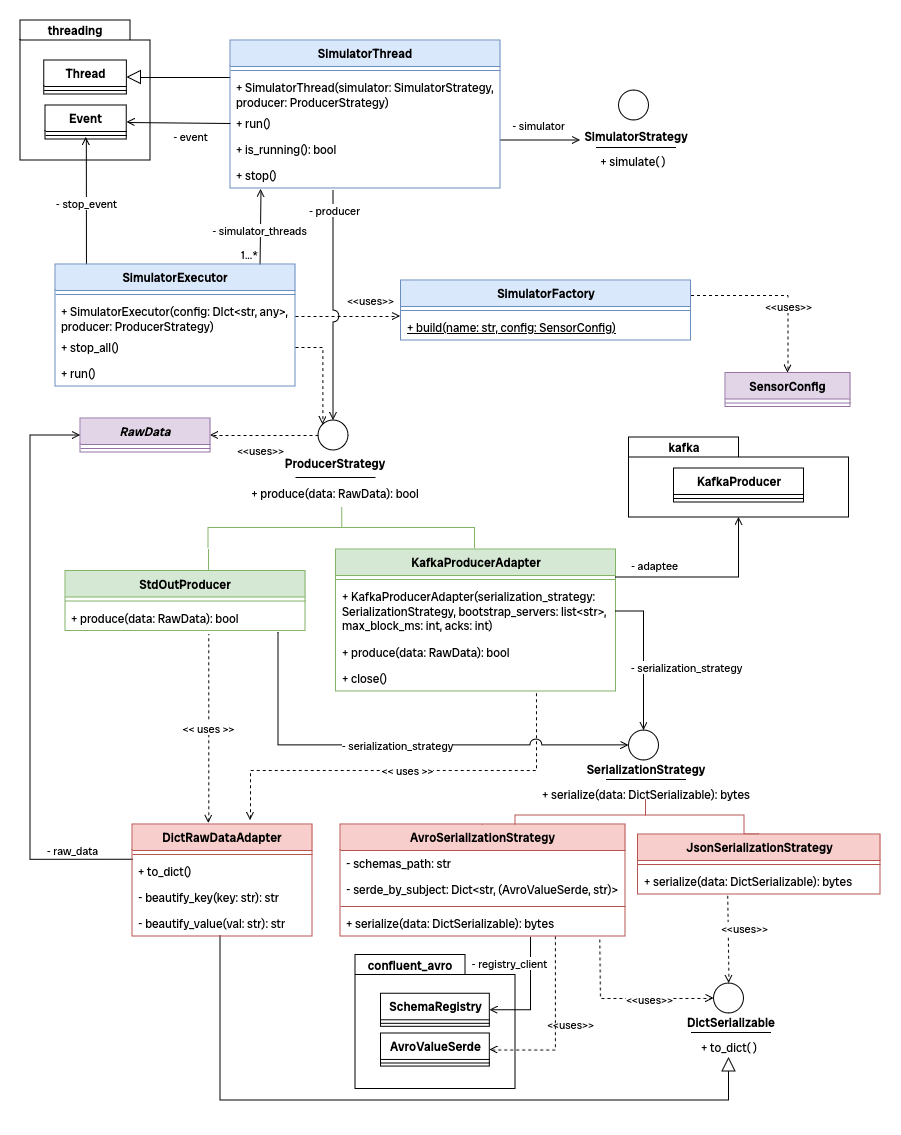
\includegraphics[width=0.87\textwidth]{./specifica_tecnica/producers_serializers.png}
	\captionof{figure}{Diagramma delle classi modulo \texttt{producers} e \texttt{serializers}}
\end{center}

\subsubsubsection{Classi, interfacce metodi e attributi}
\begin{itemize}
	\item \textbf{Interfaccia SerializationStrategy}
	      \begin{itemize}
		      \item \textbf{Metodi}:
		            \begin{itemize}
			            \item \texttt{serialize(data: DictSerializable)} bytes [public]: metodo che serializza i dati grezzi in \textit{byte}.
		            \end{itemize}
	      \end{itemize}
	\item \textbf{Interfaccia DictSerializable}
	      \begin{itemize}
		      \item \textbf{Metodi}:
		            \begin{itemize}
			            \item \texttt{to\_dict()} dict [public]: metodo che restituisce un dizionario Python.
		            \end{itemize}
	      \end{itemize}
	\item \textbf{Classe AvroSerializationStrategy}
	      \begin{itemize}
		      \item \textbf{Attributi}:
		            \begin{itemize}
			            \item \texttt{schemas\_path} str [private]: percorso della cartella contenente gli schemi Avro;
			            \item \texttt{registry\_client} SchemaRegistry [private]: client per interagire con lo schema registry, contenuto nella libreria \texttt{confluent\_avro};
			            \item \texttt{serde\_by\_subject} Dict[str, (AvroValueSerde, str)] [private]: \textit{cache} per memorizzare gli oggetti \texttt{AvroValueSerde} e gli schemi Avro associati.
		            \end{itemize}
		      \item \textbf{Metodi}:
		            \begin{itemize}
			            \item \texttt{serialize(data: DictSerializable)} bytes [public]: serializza i dati grezzi in \textit{byte} utilizzando il formato Confluent Avro.
		            \end{itemize}
	      \end{itemize}
	\item \textbf{Classe DictRawDataAdapter}
	      \begin{itemize}
		      \item \textbf{Metodi}:
		            \begin{itemize}
			            \item \texttt{to\_dict()} dict [public]: restituisce un dizionario Python a partire da un'istanza di \texttt{RawData};
			            \item \texttt{beautify\_key(key: str)} str [private]: formatta una chiave del dizionario;
			            \item \texttt{beautify\_value(value: object)} str [private]: formatta un valore del dizionario.
		            \end{itemize}
	      \end{itemize}
	\item \textbf{Classe JsonSerializationStrategy}
	      \begin{itemize}
		      \item \textbf{Metodi}:
		            \begin{itemize}
			            \item \texttt{serialize(data: DictSerializable)} bytes [public]:
		            \end{itemize}
	      \end{itemize}

\end{itemize}

\subsection{Redpanda}
\subsubsection{\textit{Topic}}
Nel contesto di Redpanda, un \textit{topic} è una categoria o canale a cui vengono inviati i dati. Essi sono utili per
organizzare logicamente i diversi tipi di messaggi o eventi. Nel nostro sistema, i dati grezzi provenienti dai simulatori vengono pubblicati in un \textit{topic}
differente per ciascun tipo di dato; ciò consente di elaborare in modo indipendente le varie tipologie di messaggi.

\subsubsection{Partizioni e chiavi}
I \textit{topic} possono essere suddivisi in più partizioni, le quali consentono la distribuzione del carico di lavoro tra più \textit{broker} Redpanda,
allo scopo di migliorare le prestazioni e la scalabilità. Ciascuna partizione di un \textit{topic} viene memorizzata in diversi nodi del \textit{cluster}; la numerosità
delle partizioni può essere configurata a seconda delle necessità.\\
Redpanda garantisce l'ordine degli eventi all'interno della stessa partizione, tuttavia di \textit{default} non è garantito l'ordine tra partizioni diverse.
Il partizionamento consente di elaborare i dati in parallelo, infatti i consumatori possono leggere da più partizioni contemporaneamente, distribuendo il carico computazionale e migliorando il \textit{throughput}.
Ogni messaggio pubblicato è detto \textit{record} e ha una chiave, che può essere utilizzata per determinare la partizione a cui il messaggio verrà assegnato, ed un valore,
che costituisce il vero e proprio \textit{payload}; eventi con la stessa chiave vengono inviati alla stessa partizione.\\
Nel caso del nostro progetto, abbiamo deciso di utilizzare come chiave il \texttt{sensor\_uuid}, un identificativo univoco globale per ciascun sensore, affinché i dati
siano inviati alla stessa partizione e conseguentemente elaborati nell'ordine in cui sono stati prodotti.

\subsubsection{Redpanda schema registry}
Lo \textit{schema registry} offre un archivio centralizzato per gestire e convalidare gli schemi associati ai messaggi Kafka, facilitandone la serializzazione e deserializzazione.
I produttori e consumatori dei \textit{topic} Kafka possono utilizzare questi schemi per garantire coerenza e compatibilità dei dati durante la loro evoluzione nel tempo.

\subsubsubsection{\textit{Compatibility mode}}
Le modalità di compatibilità di uno schema sono delle regole che determinano come i cambiamenti ad uno schema influiscono sulla capacità dei dati serializzati con
versioni precedenti di essere letti da versioni successive e viceversa; sono essenziali per garantire che i dati rimangano compatibili durante l'evoluzione degli schemi.
Di seguito sono descritte le principali modalità di compatibilità supportate dallo \textit{schema registry} di Redpanda:

\begin{itemize}
	\item \texttt{BACKWARD}: i consumatori che utilizzano lo schema più recente possono leggere i dati prodotti con lo schema precedente;
	\item \texttt{BACKWARD\_TRANSITIVE}: i consumatori che utilizzano lo schema più recente possono leggere i dati prodotti con tutti gli schemi precedenti;
	\item \texttt{FORWARD}: i consumatori che utilizzano lo schema precedente possono leggere i dati prodotti con lo schema più recente;
	\item \texttt{FORWARD\_TRANSITIVE}: i consumatori che utilizzano uno qualsiasi degli schemi precedenti possono leggere i dati prodotti con lo schema più recente;
	\item \texttt{FULL}: i dati prodotti con lo schema più recente possono essere letti da consumatori che utilizzano lo schema precedente e viceversa;
	\item \texttt{FULL\_TRANSITIVE}: i dati prodotti con uno qualsiasi degli schemi possono essere letti da consumatori che utilizzano qualsiasi altro schema;
	\item \texttt{NONE}: nessun controllo di compatibilità viene effettuato.
\end{itemize}
Nel progetto proposto da \textit{SyncLab S.r.L.} l'obiettivo principale è l'elaborazione dei dati in tempo reale piuttosto che di quelli storici, pertanto
è importante che i consumatori possano sempre ricevere i messaggi più recenti, anche se prodotti con un nuovo schema. Pertanto questo tipo di applicazioni beneficiano
della modalità \texttt{FORWARD}, ovvero quella che abbiamo scelto di utilizzare.

\subsubsubsection{Serializzazione dei dati}
\subsubsubsubsection{Chiavi}
Come menzionato in precedenza, si utilizza il \texttt{sensor\_uuid} per poplare il campo chiave dei \textit{record}; tale identificativo viene, prima di essere pubblicato
nel \textit{topic}, convertito a stringa e codificato in UTF-8.

\subsubsubsubsection{Valori}
% TODO: parlare di Confluent Avro, del formato di serializzazione delle chiavi e partitioning strategy e di topic name strategy <topic>-value
Il formato Avro consente di definire attraverso JSON uno schema che descriva la struttura dei dati, permettendo di serializzare e deserializzarli in modo affidabile; la serializzazione tramite
Avro produce dati binari compatti, che consentono di ridurre l'\textit{overhead} di rete e migliore le prestazioni di trasmissione dei dati.
Solamente i dati che rispettano lo schema definito possono essere inviati nel \textit{topic}, garantendo la coerenza dei dati e facilitando la gestione delle evoluzioni dello schema.\\
Per la serializzazione dei valori abbiamo stabilito di utilizzare il formato Confluent Avro; la principale differenza rispetto al formato Avro standard è l'inclusione di un \textit{magic byte}
e dell'ID dello schema all'inizio del messaggio, seguiti dal \textit{payload} vero e proprio. Ciò consente di evitare di includere lo schema all'interno di ogni messaggio, riducendo la dimensione dei dati trasmessi.\\
Il produttore consulta lo \textit{schema registry} per ottenere l'ID corretto da utilizzare quando invia un messaggio, mentre il consumatore lo utilizza per ottenere lo schema con
cui deserializzare il messaggio.

\subsubsubsection{Formato dei messaggi}
\subsubsubsubsection{Dati grezzi prodotti dai simulatori}
Per ciascun \textit{topic} è stato definito uno schema Avro che descrive la struttura dei dati grezzi generati dai simulatori. Rispetto all'utilizzo di uno schema comune per tutti i \textit{topic},
questa scelta consente di:
\begin{itemize}
	\item rendere \textbf{indipendenti} i vari tipi di messaggi. Se una tipologia sensore dovesse cambiare il formato dei dati, sarebbe sufficiente modificare lo schema relativo al \textit{topic} corrispondente;
	\item non dover stabilire a priori il \textbf{numero di misurazioni} che un sensore può effettuare. Se si utilizzasse uno schema comune, sarebbe necessario prevedere un numero massimo di campi, anche se non tutti i sensori potrebbero utilizzarli;
	\item far conoscere al consumatore il \textbf{tipo esatto} del dato che riceverà, senza dover utilizzare un campo di tipo \textit{union}. Le misurazioni effettuate dai sensori possono essere numeri interi, decimali, stringhe o booleani;
\end{itemize}
\pagebreak
I sensori inviano, oltre alle misurazioni relative alla propria tipologia, i campi contenuti nella seguente tabella:
\begin{table}[ht]
	\begin{tabular}{lll}
		\textbf{Campo}        & \textbf{Tipo} & \textbf{Descrizione}                                     \\
		\texttt{sensor\_uuid} & string        & Identificativo univoco del sensore.                      \\
		\texttt{sensor\_name} & string        & Nome del sensore.                                        \\
		\texttt{latitude}     & double        & Latitudine del sensore.                                  \\
		\texttt{longitude}    & double        & Longitudine del sensore.                                 \\
		\texttt{timestamp}    & string        & Data e ora della misurazione in formato ISO 8601.        \\
		\texttt{group\_name}  & string        & Nome (opzionale) del gruppo di sensori a cui appartiene. \\
	\end{tabular}
\end{table}
\\
Un esempio di schema Avro per il tipo di dato \texttt{Temperature} è il seguente:
\begin{lstlisting}[language=json, caption=Esempio di schema Avro per il tipo di dato \texttt{Temperature},captionpos=b]
{
  "type": "record",
  "name": "Temperature",
  "fields": [
    { "name": "sensor_uuid", "type": "string" },
    { "name": "sensor_name", "type": "string" },
    { "name": "latitude", "type": "double" },
    { "name": "longitude", "type": "double" },
    { "name": "timestamp", "type": "string" },
    { "name": "value", "type": "float" },
    { "name": "group_name", "type": [ "string", "null" ] }
  ]
}
\end{lstlisting}

\subsubsubsubsection{Dati elaborati da Apache Flink}
Per quanto riguarda invece i dati aggregati da Apache Flink, è stato definito uno schema Avro per ciascuno di essi, il quale viene pubblicato in un \textit{topic} dedicato.
Lo schema Avro per il tipo di dato \texttt{HeatIndex} è il seguente:
\begin{lstlisting}[language=json, caption=Schema Avro per il tipo di dato \texttt{HeatIndex},captionpos=b]
{
  "type": "record",
  "name": "Heat_Index",
  "fields": [
    {"name":"sensor_names", "type": {"type":"array", "items":"string"}},
    {"name":"group_name", "type": "string"},
    {"name":"heat_index", "type": "float"},
    {"name":"avg_temperature", "type": "float"},
    {"name":"avg_humidity", "type": "float"},
    {"name":"center_of_mass_latitude", "type": "float"},
    {"name":"center_of_mass_longitude", "type": "float"},
    {"name":"radius_in_km", "type": "float"},
    {"name":"timestamp", "type": "string"}
  ]
}

\end{lstlisting}

\begin{lstlisting}[language=json, caption=Schema Avro per il tipo di dato \texttt{ChargingEfficiency},captionpos=b]
{
  "type": "record",
  "name": "Charging_Efficiency",
  "fields": [
    { "name": "sensor_uuid", "type": "string" },
    { "name": "utilization_rate", "type": "double" },
    { "name": "efficiency_rate", "type": "double" },
    { "name": "timestamp", "type": "string" },
    { "name": "group_name", "type": "string" },
    { "name":"sensor_names", "type": { "type": "array",  "items": "string" } }
  ]
}

\end{lstlisting}

\subsubsubsection{\textit{Topic name strategy}} % TODO
TODO

\subsubsection{Inizializzazione e configurazione}
TODO: parlare dell'immagine redpanda\_init

\subsubsection{Redpanda Connect}
Redpanda Connect è una piattaforma integrata nel sistema Redpanda, progettata per facilitare l'integrazione e il trasferimento dei dati tra Redpanda e altre fonti o destinazioni.
Esso consente di gestire dei connettori, componenti \textit{software} che si occupano automatizzare lo spostamento dei dati da e verso Redpanda. Tali connettori si dividono in due categorie:
\begin{itemize}
	\item \textbf{\textit{source connector}}: si occupano di trasferire i dati da una sorgente esterna a Redpanda;
	\item \textbf{\textit{sink connector}}: si occupano di trasferire i dati da Redpanda a una destinazione esterna.
\end{itemize}

\subsubsubsection{\textit{Sink connector} per ClickHouse}
All'interno del progetto abbiamo utilizzato Redpanda Connect per persistere su ClickHouse i dati provenienti dai sensori pubblicati nei differenti \textit{topic}. Per
poter effettuare questa operazione è stato necessario utilizzare un \textit{sink connector}, che si occupasse di deserializzare i messaggi in formato Confluent Avro, effettuare
il \textit{parsing} dei campi di tipo \texttt{DateTime} (pubblicati come stringhe in formato \href{https://www.iso.org/iso-8601-date-and-time-format.html}{\underline{ISO 8601}})
ed infine salvare i dati in ClickHouse.\\
La documentazione relativa è consultabile al seguente \href{https://clickhouse.com/docs/en/integrations/kafka/clickhouse-kafka-connect-sink}{\underline{url}}
[Ultima consultazione 2024-07-10].\\
La configurazione di tale connettore è disponibile all'interno del \textit{repository} del progetto al percorso \texttt{redpanda/connectors/configs/clickhouse.json}.
Al fine di effettuare il \textit{parsing} delle date è stato necessario definire all'interno di tale file un \textit{transformer}, il quale si occupa di leggere il campo \texttt{timestamp}
e convertirlo in \texttt{DateTime}, tipo riconosciuto da ClickHouse.\\
La versione utilizzata è la 1.1.1, scaricabile dal seguente \href{https://github.com/ClickHouse/clickhouse-kafka-connect/releases}{\underline{url}} [Ultima consultazione 2024-07-10].\\
La configurazione del \textit{transformer} è la seguente:
\begin{lstlisting}[language=json, caption=Configurazione del \textit{transformer} all'interno del file \texttt{clickhouse.json},captionpos=b]
{
    //...
    "transforms": "TimestampConverter",
    "transforms.TimestampConverter.type": "org.apache.kafka.connect.transforms.TimestampConverter$Value",
    "transforms.TimestampConverter.format": "yyyy-MM-dd'T'HH:mm:ss",
    "transforms.TimestampConverter.field": "timestamp",
    "transforms.TimestampConverter.target.type": "Timestamp"
    //...
}
\end{lstlisting}
La creazione del connettore viene effettuata eseguendo il seguente comando nella radice del progetto:
\begin{verbatim}
curl "localhost:8083/connectors" -H 'Content-Type: application/json' \
    -d @./redpanda/connectors/configs/clickhouse.json
\end{verbatim}

\subsubsubsection{Avro converter}
È stato inoltre necessario utilizzare un ulteriore \textit{plugin}, \texttt{avro-converter} (versione 7.6.1), scaricabile dal seguente
\href{https://www.confluent.io/hub/confluentinc/kafka-connect-avro-converter}{\underline{url}} [Ultima consultazione 2024-07-10],
il quale consente di effettuare la deserializzazione dei messaggi in formato Confluent Avro.\\
Il \textit{connector sink} è stato configurato per utilizzarlo come segue:
\begin{lstlisting}[language=json, caption=Utilizzo del \textit{plugin} \texttt{avro-converter} all'interno del file \texttt{clickhouse.json},captionpos=b]
{
    //...
    "value.converter": "io.confluent.connect.avro.AvroConverter",
    "value.converter.schemas.enable": "true",
    "value.converter.schema.registry.url": "http://redpanda:8081",
    //...
}
\end{lstlisting}

\subsubsection{Redpanda Console}
Redpanda Console è un'applicazione web che consente di gestire e effettuare \textit{debug} di un'istanza Redpanda. Essa ha diverse funzionalità, tra cui:
%
\begin{itemize}
	\item \textbf{visualizzazione dei messaggi}: consente di esplorare i messaggi dei \textit{topic} attraverso query ad-hoc e filtri dinamici, scritti con semplici funzioni JavaScript;
	\item \textbf{gruppi di consumatori}: permette di visualizzare tutti i gruppi di consumatori attivi, insieme ai relativi offset, modificarli o eliminarli;
	\item \textbf{panoramica dei \textit{topic}}: permette di visualizzare la lista dei \textit{topic}, controllarne la configurazione, lo spazio utilizzato, la lista dei consumatori e i dettagli delle partizioni;
	\item \textbf{panoramica del \textit{cluster}}: permette di visualizzare le ACL, i \textit{broker} disponibili, il loro spazio utilizzato, l'ID del rack e altre informazioni per ottenere una panoramica del \textit{cluster};
	\item \textbf{schema registry}: permette di visualizzare tutti gli schemi Avro, Protobuf o JSON all'interno del registro degli schemi;
	\item \textbf{Kafka Connect}: permette di gestire i connettori da più \textit{cluster} di connessione, modificare le configurazioni, visualizzare lo stato corrente o riavviare i task.
\end{itemize}

\subsection{Apache Flink - \textit{Processing layer}}
Nel contesto di Apache Flink, un \textit{job} è un'applicazione che definisce una serie di operazioni di trasformazione su un flusso di dati.
Essi possono essere eseguiti su \textit{cluster} distribuiti per sfruttare la scalabilità e la potenza di calcolo necessaria per elaborare grandi quantità di dati in tempo reale.
Tipicamente, un \textit{job} consiste di tre componenti principali:
\begin{itemize}
	\item \textbf{sorgente di dati (\textit{source})}: il punto di ingresso del flusso di dati, ad esempio un \textit{topic} Kafka o un file di log;
	\item \textbf{transformations}: operazioni come map, filter, aggregate, join, che trasformano i dati in ingresso;
	\item \textbf{\textit{sink}}: il punto di uscita dove i dati elaborati vengono scritti, ad esempio un database o un altro \textit{topic} Kafka.
\end{itemize}
Flink offre due API per la definizione dei \textit{job}: \textit{DataStream API} e \textit{Table API}
Il primo consente di lavorare con \textit{stream} di dati, avendo un controllo più fine sul flusso di dati, mentre il secondo permette di lavorare con tabelle, offrendo una sintassi più simile a SQL.\\
Per questo progetto abbiamo utilizzato le \textit{DataStream API} per la realizzazione di due \textit{job} indipendenti tra loro, che tuttavia condividono alcune classi di utilità.

\subsubsubsection{\textit{Heat Index}}
A partire dai dati rilevati dai sensori di temperatura e umidità relativa lo \textit{Heat Index} consente di stimare la percezione della temperatura da parte dell'essere umano.
Nella configurazione di ciascun simulatore, oltre a posizione e identificativo dello stesso, è possibile specificare un \texttt{group\_name}, ovvero una stringa che identifica
il gruppo o zona di appartenenza; si suppone che sensori situati in posizioni geografiche vicine abbiano lo stesso \texttt{group\_name}. Il \textit{job} calcola prima separatamente
la temperatura e l'umidità media per finestre di un'ora, aggregando i dati provenienti da sensori dello stesso gruppo. Successivamente con i valori ottenuti computa lo \textit{Heat Index},
utilizzando la \underline{\href{https://www.ncbi.nlm.nih.gov/pmc/articles/PMC3801457/}{formula empirica ideata da Blazejczyk}} [Ultima consultazione 2024-06-25].
Nel risultato finale, oltre al valore dello \textit{Heat Index}, vengono restituiti anche i valori di temperatura e umidità medi, il centro di massa del gruppo di sensori
(utilizzando la formula \underline{\href{https://en.wikipedia.org/wiki/Haversine_formula}{Haversine}} [Ultima consultazione 2024-06-25] per il calcolo della distanza) e la
distanza dal centro di massa al sensore più lontano. Questi ultimi due dati sono impiegati in una mappa interattiva su Grafana per poter disegnare un cerchio,
rappresentante la zona di influenza del gruppo di sensori.

\subsubsubsubsection{Modello di calcolo}
\subsubsubsubsubsection{Heat Index}
Lo \textit{Heat Index} viene calcolato con la seguente formula, dove $T$ è la temperatura in gradi Celsius, $R$ l'umidità relativa in percentuale:
\[
	HI = c_1 + c_2 T + c_3 R + c_4 TR + c_5 T^2 + c_6 R^2 + c_7 T^2 R + c_8 TR^2 + c_9 T^2 R^2
\]
e i coefficienti $c_i$ sono:
\[
	\begin{aligned}
		c_1 & = -8.78469475556          & \quad c_2 & = 1.61139411            & \quad c_3 & = 2.33854883889         \\
		c_4 & = -0.14611605             & \quad c_5 & = -0.012308094          & \quad c_6 & = -0.0164248277778      \\
		c_7 & = 2.211732 \times 10^{-3} & \quad c_8 & = 7.2546 \times 10^{-4} & \quad c_9 & = -3.582 \times 10^{-6}
	\end{aligned}
\]
\subsubsubsubsubsection{Centro di massa o centroide}
Il calcolo del centro di massa tiene in considerazione la sfericità della Terra. Sia dato un insieme di punti $P = \{(a_1, b_1), (a_2, b_2), \ldots, (a_n, b_n)\}$, dove $a_i$ rappresenta
la latitudine del punto $i$-esimo e $b_i$ la longitudine. Per calcolare il centro di massa si procede, per ciascun punto, a convertire in radianti le coordinate:
\[
	\begin{align*}
		lat_i = \frac{\pi}{180} \cdot a_i, & \quad lon_i = \frac{\pi}{180} \cdot b_i
	\end{align*}
\]
Successivamente si calcolano i coefficienti $x_i$, $y_i$ e $z_i$:
\[
	\begin{align*}
		x_i = \cos(lat_i) \cdot \cos(lon_i),       &
		\quad y_i = \cos(lat_i) \cdot \sin(lon_i), &
		\quad z_i = \sin(lat_i)
	\end{align*}
\]
Una volta ottenuti i coefficienti per tutti i punti, si calcola la media di tutti i coefficienti:
\[
	\begin{aligned}
		x & = \frac{1}{n} \sum_{i=1}^{n} x_i, & \quad y = \frac{1}{n} \sum_{i=1}^{n} y_i, & \quad z = \frac{1}{n} \sum_{i=1}^{n} z_i
	\end{aligned}
\]
Infine si calcolano $lat$ (latitudine in radianti), $lon$ (longitudine in radianti) e $hyp$ (ipotenusa ne piano cartesiano, che rappresenta la distanza dall'origine alla proiezione del punto sul piano $lat_i, lon_i$):
\begin{align*}
	lon = atan2(y, x)      \\
	hyp = \sqrt{x^2 + y^2} \\
	lat = atan2(z, hyp)
\end{align*}
Una volta ottenuti $lat$ e $lon$, si convertono in gradi e si ottiene il centro di massa $CM = (c_a, c_b)$.
\[
	\begin{align*}
		c_a = \frac{180}{\pi} \cdot lat, & \quad c_b = \frac{180}{\pi} \cdot lon
	\end{align*}
\]
\subsubsubsubsubsection{Raggio del cerchio}
Il raggio del cerchio viene calcolato come la distanza dal centro di massa al punto più lontano. Sia $P = \{(a_1, b_1), (a_2, b_2), \ldots, (a_n, b_n)\}$ l'insieme di punti, $CM = (c_a, c_b)$, il
raggio $r$ è dato da:
\[
	r = \max_{i=1}^{n} haversine(c_a, c_b, a_i, b_i)
\]


\subsubsubsubsection{Flusso di dati}
TODO: aggiungere schema flusso dati
\subsubsubsubsection{Architettura}
TODO: aggiungere schema classi + design pattern + metodi
\subsubsubsubsection{\textit{Deployment}}
TODO

\subsubsubsection{\textit{Charging Efficiency} (efficienza delle colonnine elettriche)}
A partire dai dati rilevati dai sensori di occupazione dei parcheggi e delle colonnine elettriche, questo \textit{job} calcola giornalmente per ciascun sensore i seguenti valori:
\begin{itemize}
	\item \texttt{utilization\_rate}: percentuale di tempo in cui le colonnine sono utilizzate rispetto al tempo totale considerato;
	\item \texttt{efficiency\_rate}: percentuale di tempo in cui le colonnine sono utilizzate rispetto al tempo totale in cui il parcheggio è occupato.
\end{itemize}

\subsubsubsubsection{Modello di calcolo}
TODO: spiegare come vengono calcolati i coefficienti

\subsubsubsubsection{Flusso di dati}
TODO: aggiungere schema flusso dati

\subsubsubsubsection{Architettura}
TODO: aggiungere schema classi + design pattern + metodi

\subsection{Database ClickHouse}
% Come detto in precedenza, il database adottato è \textit{ClickHouse}. Per ogni sensore è stata creata una tabella \textit{MergeTree}, che permette di memorizzare i dati in modo efficiente e di eseguire query complesse in modo veloce.

\subsubsection{Funzionalità utilizzate}
\subsubsubsection{Materialized View}
Sono una potente funzionalità di \textit{ClickHouse} per migliorare le prestazioni delle query e semplificare l'analisi dei dati. In sostanza, una materialized view è una vista pre-calcolata o una copia di una query, memorizzata fisicamente su disco in forma tabellare. Ciò consente di evitare il calcolo ripetuto dei risultati della query ogni volta che viene eseguita.
\subsubsubsection*{Documentazione}
\url{https://clickhouse.com/docs/en/guides/developer/cascading-materialized-views}

[Ultima consultazione 2024-06-05]

\subsubsubsection*{Utilizzi}
% TODO: utilizzi nel progetto
% \begin{itemize}
% 	\item \textbf{Aggregazioni pre-calcolate}: le materialized view possono essere utilizzate per memorizzare i risultati di aggregazioni complesse, come somme, medie, conteggi, ecc., in modo che non debbano essere calcolati ogni volta che viene eseguita una query;
% 	\item \textbf{rapporti pre-calcolati}: possono essere utilizzate per memorizzare i risultati di query complesse o di rapporti, in modo che i risultati siano immediatamente disponibili senza dover eseguire la query ogni volta;
% 	\item \textbf{join ottimizzati}: possono essere utilizzate per memorizzare i risultati di join complessi tra più tabelle, in modo che i risultati siano immediatamente disponibili senza dover eseguire il join ogni volta;
% 	\item \textbf{filtraggio e selezione efficiente}: possono essere utilizzate per filtrare e selezionare dati in base a criteri specifici, migliorando le prestazioni delle query che richiedono l'accesso solo a una parte dei dati.
% 	\item \textbf{Analisi dei dati storici}: i dati storici vengono memorizzati in tabelle MergeTree per consentire l'analisi e l'elaborazione dei dati storici;
% 	\item \textbf{applicazioni di business intelligence}: i dati vengono memorizzati in tabelle MergeTree per consentire l'analisi e la generazione di report per le applicazioni di business intelligence;
% 	\item \textbf{log e monitoraggio}: i dati di log e di monitoraggio vengono memorizzati in tabelle MergeTree per consentire l'analisi e il monitoraggio delle attività di sistema.
% \end{itemize}
\subsubsubsection{MergeTree}
MergeTree è uno dei principali motori di archiviazione di ClickHouse, progettato per gestire grandi volumi di dati e fornire elevate prestazioni di lettura e scrittura. È particolarmente adatto per applicazioni in cui i dati vengono aggiunti in modo incrementale e le query vengono eseguite su intervalli di tempo specifici.
Le caratteristiche principali sono:
\begin{itemize}
	\item \textbf{partizionamento}, in cui i dati vengono partizionati in base a una colonna di data o di tempo, in modo che i dati più recenti siano memorizzati in partizioni separate e possano essere facilmente eliminati o archiviati;
	\item \textbf{ordine dei dati}, dove i dati vengono ordinati in base a una colonna di ordinamento, in modo che i dati siano memorizzati in modo sequenziale e possano essere letti in modo efficiente;
	\item \textbf{indice primario}, tramite il quale i dati vengono indicizzati in base a una colonna di chiave primaria, in modo che le query di ricerca e di join siano veloci ed efficienti;
	\item \textbf{merging dei dati}, in questo modo i dati vengono uniti in modo incrementale in background, in modo che le query di aggregazione e di analisi siano veloci ed efficienti;
	\item \textbf{compressione}, i dati vengono compressi in modo efficiente per ridurre lo spazio di archiviazione e migliorare le prestazioni di lettura e scrittura;
	\item \textbf{replica e distribuzione}, i dati possono essere replicati e distribuiti su più nodi per garantire l'affidabilità e la disponibilità del sistema.
\end{itemize}
\subsubsubsection*{Documentazione}
\url{https://clickhouse.com/docs/en/engines/table-engines/mergetree-family/mergetree}

[Ultima consultazione 2024-06-05]

\subsubsection{Trasferimento dati tramite Materialized View}
Le Materialized View in ClickHouse sono viste che memorizzano fisicamente i risultati di una query specifica in modo da permettere un accesso rapido e efficiente ai dati pre-elaborati. Quando vengono create, le Materialized View eseguono la query definita e archiviano i risultati in una struttura di dati ottimizzata per l'accesso veloce. Questo consente di evitare il calcolo ripetuto dei risultati della query ogni volta che viene eseguita, migliorando notevolmente le prestazioni complessive del sistema. I vantaggi derivanti da questo approccio sono molteplici, tra questi troviamo:
\begin{itemize}
	\item \textbf{prestazioni ottimizzate}: grazie alla memorizzazione fisica dei risultati delle query, le Materialized View consentono un accesso rapido ai dati pre-elaborati, riducendo i tempi di risposta delle query complesse;
	\item \textbf{riduzione del carico di lavoro}: trasferendo i dati pre-elaborati in Materialized View, si riduce il carico di lavoro sul sistema sorgente, consentendo una maggiore scalabilità e riducendo il rischio di sovraccarico del sistema durante le operazioni di estrazione dei dati;
	\item \textbf{sempre aggiornate}: possono essere progettate per aggiornarsi automaticamente in risposta alle modifiche nei dati sottostanti, garantendo che i risultati siano sempre aggiornati e coerenti con lo stato attuale dei dati;
	\item \textbf{semplificazione dell'architettura}: è possibile semplificare l'architettura complessiva del sistema eliminando la necessità di eseguire query complesse e costose ogni volta che si accede ai dati.
\end{itemize}
%TODO prendere le query che creano le materialized view
\subsubsection{Misurazioni isole ecologiche}
Di seguito viene riportata la configurazione della tabella per le misurazioni delle isole ecologiche. Le misurazioni includono:
\begin{itemize}
	\item \textbf{sensor\_uuid}: identificativo univoco del sensore (formato UUID);
	\item \textbf{sensor\_name}: nome del sensore (formato String);
	\item \textbf{timestamp}: data e ora della misurazione (formato DateTime64);
	\item \textbf{latitude}: latitudine del sensore (formato Float64);
	\item \textbf{longitude}: longitudine del sensore (formato Float64);
	\item \textbf{filling\_value}: percentuale di riempimento dell'isola ecologica (formato Float32).
\end{itemize}
%TODO mettere foto della tabella isole ecologiche
\subsubsection{Misurazioni temperatura}
Di seguito viene riportata la configurazione della tabella per le misurazioni della temperatura. Le misurazioni includono:
\begin{itemize}
	\item \textbf{sensor\_uuid}: identificativo univoco del sensore (formato UUID);
	\item \textbf{sensor\_name}: nome del sensore (formato String);
	\item \textbf{timestamp}: data e ora della misurazione (formato DateTime64);
	\item \textbf{value}: valore della temperatura rilevata (formato Float32);
	\item \textbf{latitude}: latitudine del sensore (formato Float64);
	\item \textbf{longitude}: longitudine del sensore (formato Float64);
\end{itemize}
%TODO mettere foto della tabella temperatura
\subsubsection{Misurazioni traffico}
Di seguito viene riportata la configurazione della tabella per le misurazioni della traffico. Le misurazioni includono:
\begin{itemize}
	\item \textbf{sensor\_uuid}: identificativo univoco del sensore (formato UUID);
	\item \textbf{sensor\_name}: nome del sensore (formato String);
	\item \textbf{timestamp}: data e ora della misurazione (formato DateTime64);
	\item \textbf{latitude}: latitudine del sensore (formato Float64);
	\item \textbf{longitude}: longitudine del sensore (formato Float64);
	\item \textbf{vehicles}: numero di veicoli rilevati (formato Int32);
	\item \textbf{avg\_speed}: velocità media del traffico (formato Float32).
\end{itemize}
%TODO mettere foto della tabella traffico
\subsection{Grafana}
Grafana è uno strumento di analisi e monitoraggio che permette di visualizzare dati provenienti da una varietà di fonti. È sviluppato principalmente in Go e Typescript ed è noto per la sua capacità di creare dashboard personalizzabili e intuitive.
\subsubsection{Dashboard}
%metti stessa cosa del manuale utente riguardo le dashboard. 

\subsubsection{ClickHouse datasource plugin}
Il plugin ClickHouse per Grafana è un'implementazione che consente di utilizzare ClickHouse come fonte di dati per Grafana. Questo plugin facilita la connessione e l'interrogazione dei dati archiviati in ClickHouse direttamente da Grafana, permettendo di creare dashboard dinamiche e interattive.
\subsubsubsection*{Documentazione}
\url{https://grafana.com/grafana/plugins/grafana-clickhouse-datasource/}

[Ultima consultazione 2024-06-05]
\subsubsubsection{Configurazione del Datasource}
La configurazione  grafana/provisioning/datasources/default.yaml


\subsubsection{Variabili Grafana}
\subsubsubsection{Documentazione}
\url{https://grafana.com/docs/grafana/latest/dashboards/variables/}

[Ultima consultazione 2024-06-05]
\subsubsubsection*{Variabili nella dashboard principale}
Le variabili presenti nella dashboard principale sono:
\begin{itemize}
	\item \textbf{tipo sensore}: permette di selezionare il tipo di sensore da visualizzare (temperatura, traffico, isola ecologica...);
	\item \textbf{nome sensore}: permette di selezionare il nome del sensore da visualizzare (ad esempio sensore1, sensore2, ecc.); % TODO
\end{itemize}
%TODO mettere foto codice query
\subsubsubsection*{Variabili nella dashboard dettagliata}
Le variabili presenti nelle dashboard dettagliate sono:
\begin{itemize}
	\item \textbf{nome sensore}: permette di selezionare il nome del sensore da visualizzare (es. sensore1, sensore2, ecc.);
\end{itemize}

\subsubsection{Grafana Alerts}
Sono una funzionalità che permettono di definire, configurare e gestire avvisi basati su condizioni specifiche rilevate nei dati monitorati. Questi avvisi consentono agli utenti di essere informati tempestivamente su eventuali problemi o cambiamenti critici nei loro sistemi, applicazioni o infrastrutture.
\subsubsubsection*{Documentazione}
\url{https://grafana.com/docs/grafana/latest/alerting/} [Ultima consultazione 2024-06-05]
\subsubsubsection{Configurazione delle regole di alert}
Definiscono le condizioni che devono essere soddisfatte per attivare un alert. Gli eventi che generano un alert sono:
\begin{itemize}
	\item temperatura maggiore di 40°C per più di 30 minuti;
	\item isola ecologica piena al 100\% per più di 24 ore;
	\item superamento dell'indice 3 dell'EAQI (indice di qualità dell'aria);
	\item livello di precipitazioni superiore a 10 mm in 1 ora.
\end{itemize}
Gli alert possono possedere tre diversi tipi di stati:
\begin{itemize}
	\item \textbf{\textit{normal}}, indica che l'alert non è attivo perché le condizioni definite per l'attivazione dell'avviso non sono soddisfatte;
	\item \textbf{\textit{pending}}, indica che le metriche monitorate stanno iniziando a deviare dalle condizioni normali ma non hanno ancora soddisfatto completamente le condizioni per attivare l'alert;
	\item \textbf{\textit{firing}}, significa che le condizioni definite per l'avviso sono state soddisfatte e l'alert è attivo.
\end{itemize}
\subsubsubsection{Configurazione canale di notifica}
Per configurare un canale di notifica è necessario:
\begin{enumerate}
	\item nel menù di sinistra, cliccare sull'icona "Alerting";
	\item selezionare la voce "Notification channels";
	\item cliccare sul pulsante "Add channel" per aggiungere un nuovo canale di notifica;
	\item selezionare il tipo di canale di notifica desiderato tra quelli disponibili;
	\item configurare le impostazioni del canale di notifica in base alle proprie esigenze;
	\item cliccare sul pulsante "Save" per salvare le impostazioni del canale di notifica.
\end{enumerate}
% \textit{7Last} ha deciso di rendere risponibile il server \textit{Discord} configurato a questo scopo e raggiungibile a questo link:
% \begin{center}
% 	\url{https://discord.com/channels/1214553333113556992/1241974479345942568}
% \end{center}
\subsubsection{Altri plugin}
\subsubsubsection{Orchestra Cities Map plugin}
Progettato per facilitare la visualizzazione e l'analisi dei dati geospaziali all'interno di piattaforme di pianificazione urbana e sviluppo territoriale.\\
Le principali funzionalità offerte da questo plugin sono:
\begin{itemize}
	\item \textbf{visualizzazione dei dati geospaziali}: consente agli utenti di visualizzare dati geografici, come mappe, strati di dati GIS (Geographic Information System), punti di interesse e altre informazioni territoriali;
	\item \textbf{interfaccia interattiva}: offre un'interfaccia utente intuitiva e interattiva che consente agli utenti di esplorare e interagire con i dati geospaziali in modo dinamico;
	\item \textbf{personalizzazione}: offre opzioni di personalizzazione per adattarsi alle esigenze specifiche dell'utente o dell'applicazione;
	\item \textbf{analisi dei dati}: oltre alla semplice visualizzazione dei dati geospaziali, il plugin può anche supportare funzionalità avanzate di analisi dei dati, come l'identificazione di cluster, la creazione di heatmap e l'esecuzione di analisi spaziali per identificare tendenze o pattern significativi nei dati territoriali;
	\item \textbf{integrazione}: è progettato per integrarsi facilmente con altre componenti dell'ecosistema Orchestra Cities e con altre piattaforme software di pianificazione urbana e sviluppo territoriale.
\end{itemize}

\subsubsubsection*{Documentazione}
\url{https://grafana.com/grafana/plugins/orchestracities-map-panel/?tab=installation}

[Ultima consultazione 2024-06-05]
